\documentclass[paper=A4,pagesize=auto,12pt,headinclude=true,footinclude=true,BCOR=0mm,DIV=calc]{scrartcl}

\usepackage[utf8]{inputenc}
\usepackage{amsmath}
\usepackage[T1]{fontenc}
\usepackage{lmodern}
\usepackage[ngerman]{babel}
\usepackage[hidelinks]{hyperref}
\usepackage{setspace}
\usepackage[left=25mm, right=25mm, top=25mm, bottom=25mm]{geometry}
\usepackage[backend=biber, style=ieee, citestyle=ieee]{biblatex}
\usepackage[table]{xcolor}
\usepackage{graphicx}
\usepackage{wrapfig}
\usepackage{lipsum}
\usepackage[nottoc,numbib]{tocbibind}
\onehalfspacing

\bibliography{forschungsbericht}

%opening
\title{Auswirkungen eines Hintergrundes auf die Identifikation von Objekten in Bildern mithilfe eines Convolutional Neural Network}
\author{Alexandra Zarkh, Sui Yin Zhang,\\ Lennart Leggewie und Alexander Schallenberg}

\makeatletter
\def\@maketitle{%
	\newpage
	\null
	\vskip 2em%
	\begin{center}%
		\let \footnote \thanks
		{\Huge \textbf{\@title} \par}%
		\vskip 3em%
		{\large
			\lineskip .5em%
			\begin{tabular}[t]{c}%
				\@author
			\end{tabular}\par}%
		\vskip 2em%
		{\large Hochschule Bonn-Rhein-Sieg, Fachbereich Informatik, D-53757\par}%
		\vskip 2em%
		{\large \@date}%
	\end{center}%
	\par
	\vskip 1.5em}
\makeatother


\setlength{\arrayrulewidth}{0.3mm}
\setlength{\tabcolsep}{10pt}

\newcommand*\justify{%
	\fontdimen2\font=0.4em% interword space
	\fontdimen3\font=0.2em% interword stretch
	\fontdimen4\font=0.1em% interword shrink
	\fontdimen7\font=0.1em% extra space
	\hyphenchar\font=`\-% allowing hyphenation
}

\renewcommand{\texttt}[1]{%
	\begingroup
	\ttfamily
	\begingroup\lccode`~=`/\lowercase{\endgroup\def~}{/\discretionary{}{}{}}%
	\begingroup\lccode`~=`[\lowercase{\endgroup\def~}{[\discretionary{}{}{}}%
	\begingroup\lccode`~=`.\lowercase{\endgroup\def~}{.\discretionary{}{}{}}%
	\begingroup\lccode`~=`(\lowercase{\endgroup\def~}{(\discretionary{}{}{}}%
	\catcode`/=\active\catcode`[=\active\catcode`.=\active\catcode`(=\active
	\justify\scantokens{#1\noexpand}%
	\endgroup
}

\renewcommand{\listoffigures}{\begingroup
	\tocsection
	\tocfile{\listfigurename}{lof}
	\endgroup}

\renewcommand{\listoftables}{\begingroup
	\tocsection
	\tocfile{\listtablename}{lot}
	\endgroup}

\begin{document}

\begin{titlepage}
	\maketitle
\end{titlepage}

\tableofcontents
\newpage


\section{Zusammenfassung}
Im folgenden Text werden Sie ein Convolutional Neural Network, oder kurz CNN, welches in Java programmiert wurde, im Detail kennenlernen. Außerdem wird diskutiert, inwieweit  sich Hintergründe auf die Identifikation von Objekten in Bildern mithilfe eines Convolutional Neural Networks auswirken.
Im ersten Teil des Textes wird die verwendete Literatur, die Theorie und die Fragestellung vorgestellt. Anschließend folgen die Methoden. Unter anderem wird hier erklärt, was ein Convolutional Neural Network ist und wie es hier implementiert wurde. Hier werden im Detail dann die Klassen \texttt{ConvNet}, \texttt{ImageAdapter}, \texttt{TrainData} und die genutzten Testdateien vorgestellt. Der letzte Teil des Abschnitts Methoden präsentiert dann die durchgeführten Test.
Zum Schluss werden die Ergebnisse nochmal aufgeführt und zusammengefasst. Genutzte Grafiken und Tabellen findet man ebenfalls dort wieder. Daraufhin wird die Fragestellung des Berichts nochmal aufgegriffen und diskutiert. In den letzten beiden Abschnitten findet man sowohl die Literatur als auch den Anhang.


\section{Einleitung} %Alexi
Die Gesichtserkennung am Smartphone ermöglicht das Entsperren eines Gerätes und auf verschiedenen Applikationen die Nutzung von Filtern, die das Gesicht und die Umgebung erkennen und entweder die Umgebung oder bestimmte Eigenschaften und Merkmale in Gesichtern selber verändern.
Das Autofahren wird immer einfacher und komfortabler für die Person am Steuer und das hat man unter anderem der Schilder- und Fahrbahnlinienerkennung zu verdanken. Jetzt stellt sich die Frage: wie funktioniert das? Die Antwort ist ein Convolutional Neural Network.

\subsection{Verwendete Literatur}

\subsection{Theorie} %Alexi
Bedauerlicherweise treten einige Probleme bei der Verkehrszeichenerkennung auf, die nicht direkt vom Convolutional Neural Network selber ausgehen, sondern von der Umgebung. Wie zum Beispiel Schilder, die schwer zu erkennen sind, weil sie entweder schon sehr alt und dreckig sind oder zugeklebt wurden. Das erschwert dem CNN die Erkennung des Schildes und kann zu Irrtümern führen, die dann im schlimmsten Fall einen Unfall verursachen können. 
Ein weiteres Problem könnte der Verkehrsschilderwald in der Stadt sein. Dann wird es für das CNN schwerer, sich das gewollte Verkehrsschild auszusuchen, da mittlerweile sehr viele Schilder an einem Ort angebracht sind. Schwieriger wird es auch für das Convolutional Neural Network ein Verkehrsschild zu erkennen, wenn der Hintergrund sehr farbig ist und mit den Farben des Verkehrsschildes ähnelt. Dann könnte es schwierig werden, das Bild zurecht zuschneiden und die Ränder des Schildes zu erkennen.

\subsection{Fragestellung}
Die Leitfrage ist nun: Welche Auswirkungen hat ein Hintergrund eines Bildes auf die Kosten der Kalkulation eines Convolutional Neural Network (CNN), welches ein Objekt im Vordergrund des Bildes erkennen und identifizieren soll?


\section{Methoden}
Die Fragestellung wird im Folgenden am Beispiel von acht Verkehrszeichen geklärt.

\subsection{Convolutional Neural Networks} %Lennart
Ein Convolution Neural Network, auch ConvNet oder CNN genannt, ist ein Deep-Learning-Algorithmus, der ein Bild aufnimmt, verschiedenen Objekten im Bild eine Bedeutung zuweist und diese Objekte voneinander unterscheiden kann \cite{cnn1}. Das CNN ist ein mathematisches Konstrukt das normalerweise aus Schichten oder Bausteinen besteht. Die ersten beiden Schichten, Convolution und Pooling-Schicht, extrahieren bestimmte Merkmale aus einem Bild, während die dritte Schicht, vollständig verknüpfte Schicht, die extrahierten Merkmale in die endgültige Ausgabe umsetzt. Eine typische Architektur besteht aus Wiederholungen eines Stapels von mehreren Convolution-Schichten und einer Pooling-Schicht gefolgt von mehreren vollständig verknüpften Schichten. Der Vorgang, bei dem die Eingabedaten durch diese Schichten in Ausgabedaten umgewandelt werden, wird als Vorwärtspropagation bezeichnet. Die in diesem Abschnitt erläuterten Convolution und Pooling-Operationen beziehen sich jedoch auf ein 2D-CNN, ähnliche Operationen können aber auch für 3D-CNN durchgeführt werden.\cite{cnn2}

\subsubsection{Convolution}
Convolution ist eine lineare Operation, die für die Merkmalsextraktion verwendet wird. Um bestimmte Merkmale zu extrahieren wird ein Array, der sogenannte Kernel, auf das Eingabe-Bild, das auch zu einem Array umgewandelt wurde, namens Kernel, angewendet.\\
Ein elementweises Produkt zwischen jedem Element des Kernels und dem Eingabetensor wird an jeder Stelle des Tensors kalkuliert und summiert, um den Ausgabewert an der zugehörigen Stelle des Ausgabetensors, einer so genannten Merkmalskarte, zu erhalten. Dieses Verfahren wird unter Anwendung mehrerer Kernel wiederholt, um eine beliebige Anzahl von Merkmalskarten zu erzeugen, die jeweils verschiedene Merkmale des Eingabetensors darstellen.\\
\begin{wrapfigure}{r}{0.5\textwidth}
	\centering
	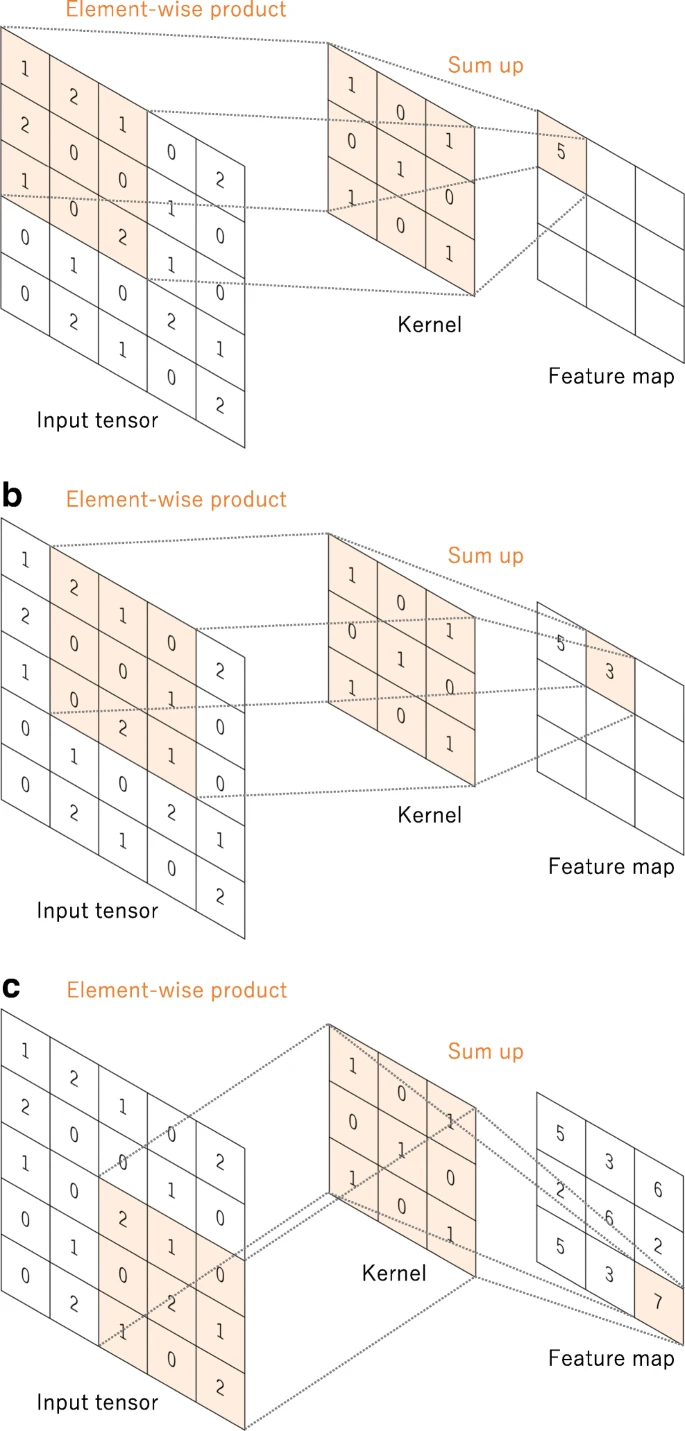
\includegraphics[width=6cm]{"images/cnn.png"}
	\caption{Benutzung des Kernels}
	\label{useofkernel}
\end{wrapfigure}
Die hier beschriebene Convolution-Operation lässt nicht zu, dass die Mitte eines Kernels das äußerste Element des Eingabetensors überdeckt, und verringert somit die Höhe und Breite der Merkmalskarte. Das Auffüllen mit Nullen ist eine Technik zu Lösung dieses Problems, bei der Zeilen und Spalten mit Nullen auf jeder Seite des Eingabetensors angefügt werden, so dass das Zentrum eines Kernels auf das äußerste Element passt und die gleiche Dimension in der Ebene durch die Convolution-Operation beibehalten wird. Der Abstand zwischen zwei aufeinanderfolgenden Kernelpositionen wird als Stride bezeichnet, der auch die Convolution-Operation definiert. Üblicherweise wird ein Stride der Größe 1 gewählt, jedoch wenn man ein Downsampling  der Merkmalskarten erreichen möchte, wird ein Stride größer als 1 verwendet.

\subsubsection{Pooling-Schicht}
Eine Pooling-Schicht bietet eine klassische Downsampling-Operation, die die Dimensionalität der Merkmalskarten in der Ebene reduziert, um eine Übersetzungsinvarianz gegenüber kleinen Verschiebungen und Verzerrungen einzuführen und die Anzahl der nachfolgenden lernbaren Parameter zu verringern. Es ist hervorzuheben, dass es in keiner der Pooling-Schichten einen lernbaren Parameter gibt, während Filtergröße, Stride und Padding Hyperparameter bei Pooling-Operationen sind, ähnlich wie bei Convolution-Operationen.\cite{cnn2}

\subsubsection{Max Pooling}
Die gängigste Form der Pooling-Operation ist das Max-Pooling, bei dem aus den eingegebenen Merkmalskarten Felder extrahiert werden, der maximale Wert in jedem Feld ausgegeben und alle anderen Werte verworfen werden. Üblicherweise wird ein Filter der Größe 2 x 2 mit einem Stride von 2 verwendet. Dadurch wird die In-Plane-Dimension der Merkmalskarte um den Faktor 2 verkleinert.\cite{cnn2}

\subsubsection{Global Average Pooling}
Eine weitere erwähnenswerte Pooling-Operation ist das Global Average Pooling, dass eine extreme Art des Downsamplings durchführt. Hierbei wird eine Merkmalskarte mit einer Größe von Höhe x Breite in ein 1 x 1 Array verkleinert, indem der Durchschnitt aller Elemente in jeder Merkmalskarte gebildet wird, während die Tiefe der Merkmalskarte erhalten bleibt. In der Regel wird dieser Vorgang nur einmal vor den vollständig verknüpften Schichten durchgeführt. Der erste Vorteil des Global Average Pooling’s ist, dass die Anzahl der lernbaren Parameter reduziert wird und der zweite Vorteil ist, dass das CNN Eingaben variabler Größe akzeptieren kann.\cite{cnn2}

\subsubsection{Vollständig Verknüpfte Schicht}
Die Ausgangsmerkmalskarten der letzten Convolution oder Pooling-Schicht werden in der Regel abgeflacht, das heißt in ein eindimensionales Zahlenfeld umgewandelt und mit einer oder mehreren vollständig verknüpften Schichten, auch als dichte Schichten bekannt, verbunden, in der jeder Eingang mit jedem Ausgang durch ein lernbares Gewicht verbunden ist. Sobald die von den Convolution-Schichten extrahierten und von den Pooling-Schichten heruntergestuften Merkmale erstellt sind, werden sie von einer Untergruppe vollständig verknüpften Schichten auf die endgültigen Ausgaben des Netzes abgebildet, zum Beispiel die Wahrscheinlichkeiten für jede Klasse bei Klassifizierungsaufgaben. Die letzte vollständig verknüpfte Schicht hat in der Regel die gleiche Anzahl von Ausgangsknoten wie die Anzahl der Klassen.\cite{cnn2}


\subsection{Implementierung} %Sui Yin
Die Implementierung in Java 17 besteht aus den vier neuen Klassen \texttt{ImageAdapter}, \texttt{ConvNet}, \texttt{RoadSignLabel}, \texttt{RoadSignTest} und einem Record \texttt{TrainData}. Zum Testen wird eine weitere Klasse und ein Enum verwendet. Diese vier neuen Klassen, das Record sowie die Testdateien werden im Folgenden Absätzen erklärt.

\subsubsection{ConvNet} %Alex
Die Klasse \texttt{ConvNet} soll ein Convolutional Neural Network darstellen und erbt daher von der im Projektbericht \cite{projektbericht} unter Abschnitt 2 genannten Klasse \texttt{Network}, was jener die gleichen Eigenschaften verleiht. Des Weiteren besitzt sie eine \texttt{java.util.ArrayList} vom Generic-Typ \texttt{TrainData} und einen \texttt{ImageAdapter} als private konstante Attribute. Erstere dient dem Speichern von Trainingsdatensätzen, die dann mit dem Aufrufen der überladenen Methode \texttt{train(double, int)} benutzt werden. Diese ruft die originale Instanz-Methode \texttt{train(double[][], double[][], double, int)} der Klasse \texttt{Network} mit den Daten aus der \texttt{ArrayList} auf.
Außerdem bietet die Klasse \texttt{ConvNet} die Instanz-Methode \texttt{addTrainData(String, int[])} um dieser Trainingsdatensätze hinzuzufügen. Diese nimmt einen Dateinamen von einem Bild und einen ganzzahligen Zielvektor. Zwei private nicht-statische Hilfsmethoden \texttt{getImages()} und \texttt{getTargets()} dienen der besseren Handhabung der \texttt{ArrayList}.\\
Die Klasse erstellt durch den Konstruktor \texttt{ConvNet(String, int, int, int, int[])} (Pfad zum Ordner mit den Bildern, gewünschte Bildweite, -höhe, Anzahl der Output-Neuronen, Anzahl der Hiddenlayers und deren Neuronen) von ihr abgeleitete Objekte.

\subsubsection{ImageAdapter} %Sui Yin
Der \texttt{ImageAdapter} ist dafür da, um das Bild zu laden und skalieren.
Die Klasse besteht aus sechs Methoden und einem Konstruktor. 
Im Konstruktor \texttt{ImageAdapter(String, int, int)} werden Pfad zu den Bildern, gewünschte Bildhöhe sowie -breite als Parameter übergeben, mit denen dann die jeweiligen Skalierungswerte für das jeweilige Bild initialisiert werden.
Die Methode \texttt{loadImage(String)} lädt das \texttt{java.awt.image.BufferedImage} mit dem übergebenen Namen und gibt es zurück.
Falls es keine Datei mit diesem Namen gibt oder diese keine Bilddatei ist, wird eine \justify{\texttt{IllegalArgumentException}} eine geworfen.
Als nächstes geht die Methode \texttt{getRGBs(BufferedImage)} alle Pixel durch und gibt deren hexadezimale RGB-Werte als Matrix für das jeweilige Bild zurück.
Die Methode \texttt{squareImage(BufferedImage)} ist dafür da, um das Bild quadratisch zuzuschneiden. 
\texttt{scaleImage(BufferedImage)} skaliert ein Bild mit einer beliebigen Höhe oder Breite.
Um ein \texttt{java.awt.image.Image} in ein \texttt{java.awt.image.BufferedImage} konvertieren, wird die Methode \texttt{convertToBufferedImage(Image)} benutzt.
In der einzigen öffentlichen Methode des \texttt{ImageAdapter}s \texttt{getImageRGBs(String)} wird mit den genannten Methoden und mithilfe eines übergebenen Dateinamens ein eindimensionales ganzzahliges Array mit allen RGB-Werten per \textit{row-major order}
\begin{equation}
	\scalebox{1.3}{$m_{ij} \rightarrow a_{64\cdot i + j}$}
\end{equation}
des aus dem Dateinamen resultierenden Bildes zurückgegeben.

\subsubsection{TrainData}
Das Record \texttt{TrainData(int[], int[])} besitzt einen Vektor mit den RGB-Werten eines Bildes und einen Zielvektor. Außerdem hat es zwei Instanz-Methoden \justify{\texttt{getImageAsDoubleArray()}} und \texttt{getTargetAsDoubleArray()}, welche die jeweiligen ganzzahligen Vektoren als Gleitkommazahl-Vektoren zurückgibt, und eine private nicht-statische Hilfsmethode \justify{\texttt{getIntAsDoubleArray(int[])}}.

\subsubsection{Test-Dateien} %Alex
Für das Testen wurden ein Enum \texttt{RoadSignLabel} und eine Klasse \texttt{RoadSignTest} implementiert. Das Enum zählt die möglichen Ergebnisse des Netzes auf, indiziert sie und kann den jeweils richtigen Zielvektor durch die Instanz-Methode \texttt{getTarget()} zurückgeben. In der Klasse befindet sich die für die Forschungsfrage relevante Main-Methode des Programms. Diese ruft eine private statische Methode \texttt{test()} in der selben Klasse auf. In dieser wird ein \texttt{ConvNet} deklariert und initialisiert, mit Datensätzen bestückt und trainiert. Dabei werden einige hilfreiche Ausgaben gemacht.

\subsection{Tests}
\rowcolors{2}{white}{lightgray}
Lorem ipsum dolor sit amet, consetetur sadipscing elitr, sed diam nonumy eirmod tempor invidunt ut labore et dolore magna aliquyam erat, sed diam voluptua. At vero eos et accusam et justo duo dolores et ea rebum. Stet clita kasd gubergren, no sea takimata sanctus est Lorem ipsum dolor sit amet. Lorem ipsum dolor sit amet, consetetur sadipscing elitr, sed diam nonumy eirmod tempor invidunt ut labore et dolore magna aliquyam erat, sed diam voluptua. At vero eos et accusam et justo duo dolores et ea rebum. Stet clita kasd gubergren, no sea takimata sanctus est Lorem ipsum dolor sit amet.
\begin{wraptable}{l}{0.5\textwidth} %l, r, c, i, o
	\centering
	\begin{tabular}{|c|c|}
		\hline
		\multicolumn{2}{|c|}{\textbf{Schildbilder im Trainingsdatensatz}}\\ \hline \hline
		\textbf{Andreaskreuz} & 5 \\ \hline
		\textbf{Fußgängerüberweg} & 6 \\ \hline
		\textbf{Gefahrenstelle} & 2 \\ \hline
		\textbf{Vorfahrt gewähren} & 5 \\ \hline
		\textbf{Vorfahrtsstraße} & 6 \\ \hline
		\textbf{Verbot der Einfahrt} & 8 \\ \hline
		\textbf{Fußgängerweg} & 8 \\ \hline
		\textbf{Stopp} & 4 \\ \hline
	\end{tabular}
	\caption{Schildbilder im Trainingsdatensatz}
	\label{trainData}
\end{wraptable}
Lorem ipsum dolor sit amet, consetetur sadipscing elitr, sed diam nonumy eirmod tempor invidunt ut labore et dolore magna aliquyam erat, sed diam voluptua. At vero eos et accusam et justo duo dolores et ea rebum. Stet clita kasd gubergren, no sea takimata sanctus est Lorem ipsum dolor sit amet. Lorem ipsum dolor sit amet, consetetur sadipscing elitr, sed diam nonumy eirmod tempor invidunt ut labore et dolore magna aliquyam erat, sed diam voluptua. At vero eos et accusam et justo duo dolores et ea rebum. Stet clita kasd gubergren, no sea takimata sanctus est Lorem ipsum dolor sit amet. Lorem ipsum dolor sit amet, consetetur sadipscing elitr, sed diam nonumy eirmod tempor invidunt ut labore et dolore magna aliquyam erat, sed diam voluptua. At vero eos et accusam et justo duo dolores et ea rebum. Stet clita kasd gubergren, no sea takimata sanctus est Lorem ipsum dolor sit amet. Lorem ipsum dolor sit amet, consetetur sadipscing elitr, sed diam nonumy eirmod tempor invidunt ut labore et dolore magna aliquyam erat, sed diam voluptua. At vero eos et accusam et justo duo dolores et ea rebum. Stet clita kasd gubergren, no sea takimata sanctus est Lorem ipsum dolor sit amet.
%\vspace{2em}
\begin{center}
	\begin{tabular}{|c|c|c|c|c|c|}
		\hline
		\multicolumn{6}{|c|}{\textbf{Anzahl Neuronen im CNN}}\\ \hline \hline
		\textbf{Input} & \textbf{Hidden 1} & \textbf{Hidden 2} & \textbf{Hidden 3} & \textbf{Hidden 4} & \textbf{Output}\\ \hline
		4096 & 64 & 64 & 64 & 64 & 8\\ \hline
	\end{tabular}
	\vspace{2em}
	\begin{tabular}{|c|c|}
		\hline
		\multicolumn{2}{|c|}{\textbf{Bildgröße}}\\ \hline \hline
		\textbf{Höhe} & \textbf{Breite}\\ \hline
		64 & 64\\ \hline
	\end{tabular}
	\vspace{2em}
	\begin{tabular}{|c|c|}
		\hline
		\multicolumn{2}{|c|}{\textbf{Training}}\\ \hline \hline
		\textbf{Lernrate} & \textbf{Wiederholungen}\\ \hline
		0.12 & 100000\\ \hline
	\end{tabular}
\end{center}



\section{Ergebnisse}



\section{Diskussion}


\printbibliography[heading=bibnumbered]


\listoffigures
\listoftables

\section{Anhang}



\end{document}
